\chapter{Experiment}\label{chap:exp}

\section{Hardware Settings}

Our experimental environment consists of one master node and ten working
nodes.
The master node is a physical machine with two quad-core CPU.
The CPU model is Intel(R) Xeon(R) CPU X5570 @ 2.93GHz.
On the other hand, each working node is a single-core physical machine.
The memory sizes are 1.5GB and 768MB, respectively.
Our management system works on the master node.
The master node also serves as a client which generate the workloads.
There are two workers on each working node.

\section{Worker Failure Tolerance}

\begin{figure}
  \resizebox{\columnwidth}{!}{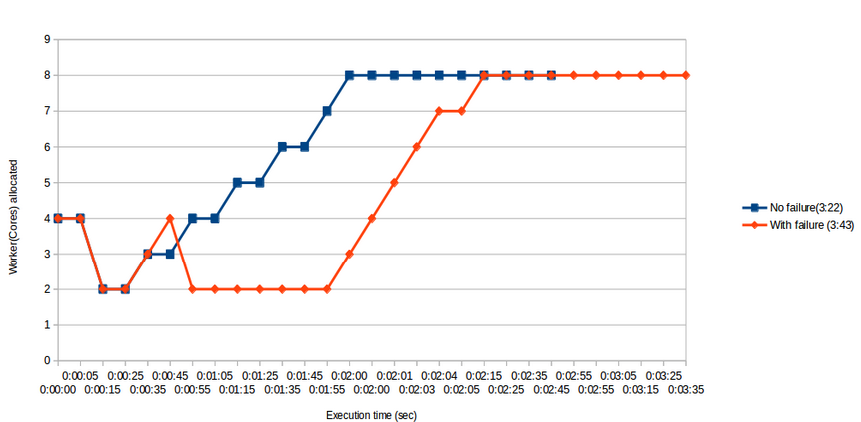
\includegraphics{figures/adaptive}}
  \caption{Worker Instance Allocation}
  \label{figure:worker-failure}
\end{figure}

We reproduced a small scale workload trace provided by Chunghwa Telecom
Laboratories~\cite{cite:cht-lab}.
Total of 8 worker instance is used and deadline-based scheduling policy
is applied in this simulation.
Only 1 job was sent and the deadline is set to 4 minutes.
The characteristic of this workload is that it starts with several
light-weight tasks and then comes with heavier tasks.

Figure~\ref{figure:worker-failure} shows the worker allocated for that
job.
The blue line is the normal execution, and the red line shows the
execution progress with workers manually shutted down to simulate worker
failure.
Six workers are manually shutted down at 0:00:55 and resumed after
0:01:55, which means at the period, only 2 workers are available.

We will discuss the normal execution (blue-line) first.
At the beginning, since we don't have any run time information, the
scheduler just use the default value (4 workers).
After few seconds, some tasks are done and the run time statistics from
\emph{status checker} shows that it seems that each task execution
progress is going faster than expected, so the system decided to
decrease the number of scheduled workers.
However, the system later found that the task execution progress had
been slowing down and current allocation might not be able to meet the
deadline, so it schedules more workers to the job.

The simulation with worker failure is similar to the normal one except
for we manually shutted down and resumed workers.
After worker resumed, the system tried harder to catch up the deadline.
We can see that the slope of the worker number change of red line is
greater than the blue line, implying the systems ability to adapt to
failure events.

\section{Trace-based Simulation}

We conducted a trace-based sleep simulation to demonstrate the
efficiency of our system.
Whenever a worker receives a task, it simply sleeps a period of time
according to the information on the received task.
Because all the worker do is simply sleeping, deploying more workers
than the number of CPUs on a single server makes extremely little impact
to the performance.

Since we could not obtain traces with deadline, we decided to use traces
in \emph{standard workload format}~\cite{cite:swf}.
The trace we use is the SDSC-Par96 log, containing 32135 jobs.
This log contains a years worth of accounting records for the 416-node
Intel Paragon located at the San Diego Supercompter Center (SDSC).
The workload logs from the SDSC Paragon were graciously provided by
Reagan Moore and Allen Downey, who also helped with background
information and interpretation.
%The trace we used are the \emph{CERIT-SC workload log}, which is
%provided by the CERIT-SC and the Czech National Grid Infrastructure
%MetaCentrum~\cite{cite:metacentrum}.
%The data set containing 17,900 jobs are generated from TORQUE traces
%during the first 3 months of the year 2013.
We took samples from these eighteen-thousand jobs, and scaled the
waiting and execution time of the sampled jobs.

\subsection{Simulation Settings}
\subsubsection{Trace Sampling}

The trace is however very sparse and skewed.
The running time distribution of the trace is very long-tailed and more
like a exponential distribution: Enormous number of jobs have quite
short running time (several seconds), while some jobs have extremely
long running time (several days).
Therefore, we scaled down the running time of jobs by factor of 0.001 to
lower the simulation time.
Besides, if we directly sample 1 percent of jobs the waiting time
between jobs can still be long --- maybe up to hours.
Because of this, we instead sample consecutive jobs only and scaled the
waiting time between jobs.
Limiting the number of jobs to sample out, we randomly pick a starting
job and take jobs consecutively after it.
The sample rate is 0.01 and the scale factor of waiting time between
jobs is 0.1.

There are still some assumptions to be made to fit our usage model.
First, we cannot obtain information about subtasks of a jobs.
So we take the processors of allocated for a job as its number of tasks
and take the total running time as the execution time of each task,
which means we assume every task in a job takes identical time to run.
Besides, the information about batches, priority and deadlines is absent
in the trace but however our targeted characteristics.
Since jobs in standard workload format traces are independent, we group
jobs that will be submitted within 1 second together to simulate
batches.
For priority, we group jobs with same user IDs as same priority and we
give the priority group with less jobs higher priority.
As for the deadlines, we use the double of its running time as deadline
for those jobs with less than 4 tasks, and for those jobs with more
tasks, we use $2 * runtime * \#task / 4$ as deadline.

During the simulation, the client starts new jobs according to the
arrival time and execution time from the trace.
Since the actual workloads is not available, a worker will be set to
``sleep mode'' after receiving a task from the client.
After resumed from the sleeping mode, the worker sends a message to the
management system indicating it has finished a task.

\subsubsection{Homogeneous/Heterogeneous Environment}

The simulation is conducted under 2 different environment settings ---
homogeneous and heterogeneous.
By homogeneous we mean each worker has identical performance.
Under this setting, when a worker received a task, it simply sleeps the
execution time marked on the task, so if 2 workers received a task
respectively from a same job, the sleeping time will be the same.
In contrast, in heterogeneous environment, workers may have different
performance.

\subsection{Experiment Results}

We evaluated the scheduling policies with two measures --- priority
violation rate and deadline miss penalty.
These measures stands for two very diverse aspect of measuring
performance of scheduling policies.
We will introduce them later respectively.
The target we compared with is the Earliest Deadline
First (EDF) algorithm, an optimal scheduling policy in real-time systems
under preemptive uni-processors.

\subsubsection{Priority Violation Rate}

In enterprise private clusters, jobs may comes in with different
priority from different users sharing the same clusters.
When the cluster resource is insufficient to satisfy all the jobs in the
system, some jobs must be sacrificed and get less resource or even
starve.
High priority ones are expected to always gain more resource than low
priority ones.
In public clusters, a cluster management system may resource to low
priority jobs rather than high ones due to different reasons such as fairness or resource utilization.
However, in enterprise clusters, priority is a very serious constraint
to satisfy.

In order to show how well a scheduling policy meets priority constraint,
we define a measure called \emph{priority violation rate}.
It is defined as $$\frac{\textrm{\#violated jobs in the
system}}{\textrm{\#jobs still in the system}}$$ and a violated job is a
job $j$ which is not scheduled with any worker while there is still at
least one job which has lower priority than $j$ but scheduled with one
or more workers.
Figure~\ref{fig:homo-violation} and~\ref{fig:hetero-violation} show the
average priority violation rate during each conducted simulation of
different scheduling policies.

\begin{figure}[htbp]
  \centering
  \includegraphics[width=\textwidth,height=0.7\textheight,keepaspectratio]{figures/homo-violation.eps}
  \caption{Average Priority Violation Rate under Homogeneous Environment}
  \label{fig:homo-violation}
\end{figure}

\begin{figure}[htbp]
  \centering
  \includegraphics[width=\textwidth,height=0.7\textheight,keepaspectratio]{figures/hetero-violation.eps}
  \caption{Average Priority Violation Rate under Heterogeneous Environment}
  \label{fig:hetero-violation}
\end{figure}

As we can see, under either homogeneous or heterogeneous environment
setting, the average violation rate of priority based policy and
deadline-based policy with spare resource filled by priority is 0, which
means there is no any priority violations.
High priority jobs are always scheduled before --- at least together
with --- low priority ones under these two policies.
In contrast to the previous two, deadline-based with spare resource
filled by deadline and EDF do not guarantee to always schedule high
priority jobs before low priority ones.
However, since EDF does not take priority into consideration, its
average violation rate is much higher (4 times as much) than
deadline-based with spare resource filled by deadline under both
homogeneous and heterogeneous environment settings.

\subsubsection{Deadline Miss Penalty}

Another aspect of measuring the performance of scheduling policies in a
system that takes (soft) deadlines into consideration is how many jobs
did not meet their deadlines and how long did they missed.
When measuring the level of the deadline missing among submitted jobs,
not only the number of jobs missed deadline, but also their priority
should be considered.
Failing to meet deadlines of high priority jobs should be penalize than
failing on low priority ones.
We used $\sum_{j \in Jobs} P_j * M_j$ as our penalty measure, where $j$
is a job of all submitted jobs, $P_j$ is the priority of $j$ and $M_j$
is the deadline missed of $j$ in seconds; we define $M_j = 0$ if a $j$
is finished before its deadline.
This measure takes both priority and deadline into consideration.
The lower the penalty score, the better the performance of the
scheduling algorithm.
The results are shown in figure~\ref{fig:homo-penalty}
and~\ref{fig:hetero-penalty}.
The shown result of each scheduling policy is the average of 5 sampled
workloads.
All of the policies used identical sample set as input benchmark.

\begin{figure}[htbp]
  \centering
  \includegraphics[width=\textwidth,height=0.7\textheight,keepaspectratio]{figures/homo-penalty.eps}
  \caption{Deadline Miss Penalty under Homogeneous Environment}
  \label{fig:homo-penalty}
\end{figure}

\begin{figure}[htbp]
  \centering
  \includegraphics[width=\textwidth,height=0.7\textheight,keepaspectratio]{figures/hetero-penalty.eps}
  \caption{Deadline Miss Penalty under Heterogeneous Environment}
  \label{fig:hetero-penalty}
\end{figure}

As we can see, EDF gives the best performance on this, either applied
under homogeneous or heterogeneous environment.
Priority-based policy and deadline-based policy with spare resource
filled by priority did not perform well --- their penalty scores are 3
magnitudes higher when compared with EDF.

Surprisingly, there is a gorgeous leap on the performance of
deadline-based policy when the spare resource is assigned to jobs with
the closest deadlines instead of the highest priorities.
The penalty score of filling by deadline is only 0.004 of filling by
priority under homogeneous environment setting, and 0.002 under
heterogeneous environment setting.

We think the main reason of this is the extremely long-tailed running
time distribution.
Despite being scaled down, the workload still contains some very
heavy-weighted jobs which takes 500 to 800 seconds.
The impact made by running time (and the relative deadlines) will be
much bigger compared with the priority scores limited under 100.
That is why the policies focused more on deadlines, such as EDF, gives
better performance.
Deadline-based policy with spare resource filled by deadline, however,
attaches more importance to priority, so it slightly underperforms EDF.
On the other hand, as we blended with the powerful EDF algorithm by
allocating spare resource with EDF, the deadline based policy has 2
magnitudes of improvement on performance compared with filling spare
resource by priority, and the performance on the deadline miss penalty
is quite close to EDF.

\subsubsection{Trade Off between the Two Measures}

In
figure~\ref{fig:homo-violation}, \ref{fig:hetero-violation}, \ref{fig:homo-penalty}
and \ref{fig:homo-penalty}, the policies more close to the right lay
more emphasis on deadline constraints, while the ones more close to the
left take priority more seriously.
We found that there is a trend that the right hand side ones performs
worse than left hand side ones (higher violation rate) on priority
violation measure, but performs well on another measure.
This somehow indicates that there is a trade off between these two
measures.

